\subsection{Mikrocontroller}\label{subsubsec:Detailkonzept_Mikrocontroller}

\subsubsection{Problem}\label{subsubsec:Problem_Mikrocontroller}

Der Mikrocontroller steuert die Prozesse und ist folglich mit den meisten Komponenten auf dem Board verbunden. Ausserdem muss er programmierbar sein, was über die SPI-Schnittstelle geschieht. Falls ein Bootloader installiert ist, benötigt es die UART-Schnittstelle. Der Mikrocontroller an sich benötigt noch ein paar andere Komponenten, die für seinen Betrieb von Wichtigkeit sind. Dazu gehören beispielsweise die Stützkondensatoren und der Oszillator.

\subsubsection{Schaltungsaufbau}\label{subsubsec:Schaltungsaufbau_Mikrocontroller}

Der Schaltungsaufbau gestaltet sich wie in Abbildung \ref{fig:Schema_Mikrocontroller} dargestellt. 

\begin{figure}[h!]
\centering
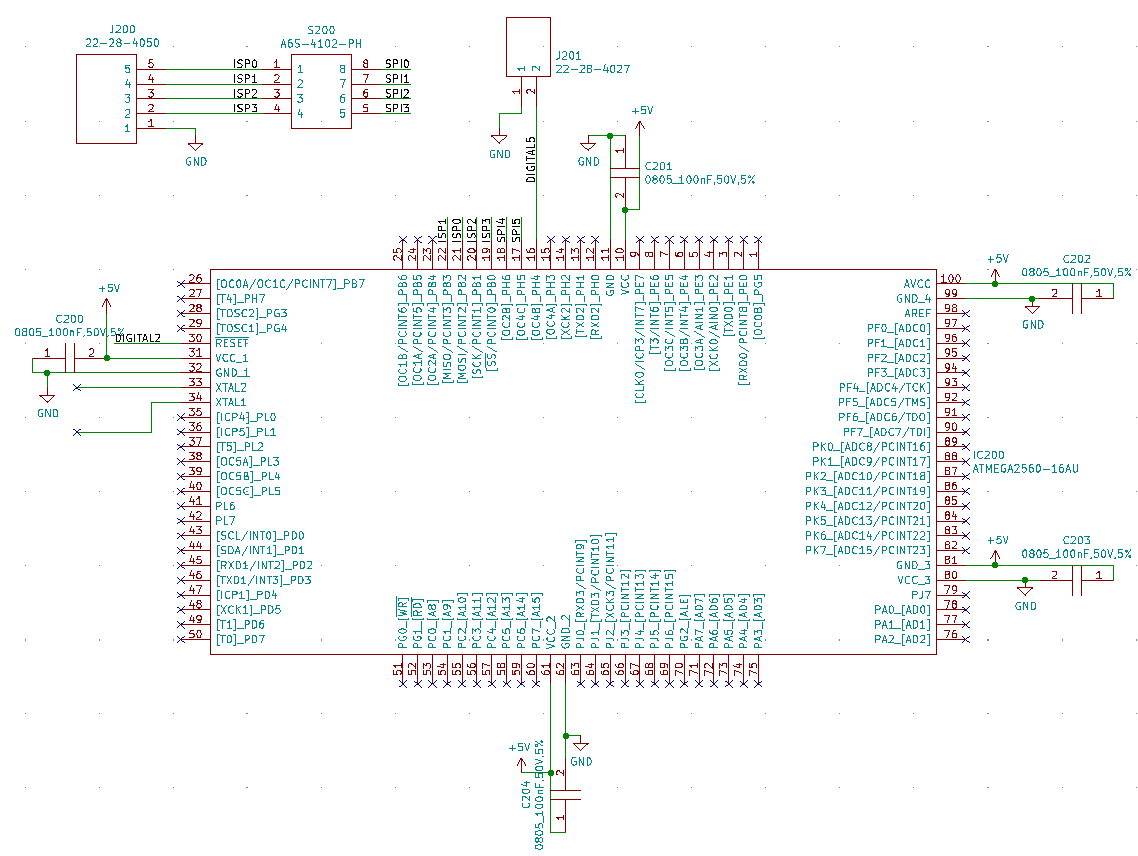
\includegraphics[width=\textwidth]{graphics/Schema_Atmega2560.png}
\caption{Schema des Mikrocontrollers}
\label{fig:Schema_Mikrocontroller}
\end{figure}
\newpage
\subsubsection{Stützkondensatoren}\label{subsubsec:Stützkondensatoren_Mikrocontroller}

\begin{tabbing}
\parbox[t]{.25\textwidth}{

Funktion

} \=\parbox[t]{.75\textwidth}{

Die Stützkondensatoren \textbf{C200 bis C204} glätten die Versorgungsspannung am Spannungseingang des Mikrocontrollers im Falle von Energiespitzen. 

}\\
\\
\parbox[t]{.25\textwidth}{

Dimensionierung

} \>\parbox[t]{.75\textwidth}{

Die Dimensionierung geschieht nach Richtwert und wurde auf 100nF festgelegt.

}\\
\\
\parbox[t]{.25\textwidth}{

Wert

} \>\parbox[t]{.75\textwidth}{

\begin{tabular}{lll}
$\mathbf{C_{Stütz}}$ & \textbf{=} &  \textbf{100nF} \\
\end{tabular}

}
\end{tabbing}

\subsubsection{Oszillator}\label{subsubsec:Oszillator_Mikrocontroller}

\begin{tabbing}
\parbox[t]{.25\textwidth}{

Funktion

} \=\parbox[t]{.75\textwidth}{

Der Oszillator \textbf{XTAL} gibt dem Mikrocontroller die Schwingung vor. Er muss eine Ausgangsfrequenz von 16MHz haben. Der ausgewählte Oszillator benötigt weiter noch zwei Kondensatoren und zu funktionieren.

}\\
\\
\parbox[t]{.25\textwidth}{

Dimensionierung

} \>\parbox[t]{.75\textwidth}{

Die Dimensionierung für den Oszillator wird vom Mikrocontroller gegeben, die Kondensatoren vom Oszillator.

}\\
\\
\parbox[t]{.25\textwidth}{

Wert

} \>\parbox[t]{.75\textwidth}{

\begin{tabular}{lll}
$\mathbf{XTAL}$ & \textbf{=} &  \textbf{16MHz} \\
$\mathbf{C_{XTAL}}$ & \textbf{=} &  \textbf{22pF} \\
\end{tabular}

}
\end{tabbing}
\todo{Funktion: Oszillator Kondensatoren/Beschriftungen anpassen}
\todo{Funktion: Oszillator Kondensatoren/Beschriftungen anpassen}

\subsubsection{UART}\label{subsubsec:UART_Mikrocontroller}

\begin{tabbing}
\parbox[t]{.25\textwidth}{

Funktion

} \=\parbox[t]{.75\textwidth}{

Die UART-Schnittstelle ist vordefiniert und benötigt keine weiteren Komponenten, um zu funktionieren. Das in den Komponenten verbaute UART-Interface ist vollständig ausgestattet.

}\\
\\
\parbox[t]{.25\textwidth}{

Dimensionierung

} \>\parbox[t]{.75\textwidth}{

Für die UART-Schnittstelle wird keine Dimensionierung benötigt.

}\\
\\
\parbox[t]{.25\textwidth}{

Wert

} \>\parbox[t]{.75\textwidth}{

Es gibt keine definierten Werte.\\

%Die Verbindungen für die SPI-Schnittstelle sind folgende:

%\begin{tabular}{lll}
%$\mathbf{UART0}$ & \textbf{=} &  \textbf{UART RX\_0} \\
%$\mathbf{UART1}$ & \textbf{=} &  \textbf{UART TX\_0} \\
%$\mathbf{UART2}$ & \textbf{=} &  \textbf{UART RX\_1} \\
%$\mathbf{UART3}$ & \textbf{=} &  \textbf{UART TX\_1} \\
%$\mathbf{UART4}$ & \textbf{=} &  \textbf{UART RX\_2} \\
%$\mathbf{UART5}$ & \textbf{=} &  \textbf{UART TX\_2} \\
%\end{tabular}


}
\end{tabbing}

\subsubsection{SPI}\label{subsubsec:SPI_Mikrocontroller}

\begin{tabbing}
\parbox[t]{.25\textwidth}{

Funktion

} \=\parbox[t]{.75\textwidth}{

Die SPI-Schnittstelle ist vordefiniert und benötigt keine weiteren Komponenten, um zu funktionieren. Das in den Komponenten verbaute SPI-Interface ist vollständig ausgestattet. Es wäre möglich Pull-Up-Widerstände zu verbauen, im Falle der Cocktailmaschine wird jedoch darauf verzichtet.

}\\
\\
\parbox[t]{.25\textwidth}{

Dimensionierung

} \>\parbox[t]{.75\textwidth}{

Für die SPI-Schnittstelle wird keine Dimensionierung benötigt.

}\\
\\
\parbox[t]{.25\textwidth}{

Wert

} \>\parbox[t]{.75\textwidth}{

Es gibt keine definierten Werte.\\

%Die Verbindungen für die SPI-Schnittstelle sind folgende:

%\begin{tabular}{lll}
%$\mathbf{SPI0}$ & \textbf{=} &  \textbf{SPI MOSI} \\
%$\mathbf{SPI1}$ & \textbf{=} &  \textbf{SPI MISO} \\
%$\mathbf{SPI2}$ & \textbf{=} &  \textbf{SPI CLK} \\
%$\mathbf{SPI3}$ & \textbf{=} &  \textbf{SPI TMC4671} \\
%$\mathbf{SPI4}$ & \textbf{=} &  \textbf{SPI EEPROM} \\
%$\mathbf{SPI5}$ & \textbf{=} &  \textbf{SPI TMC6200} \\
%\end{tabular}


}
\end{tabbing}

\subsubsection{ISP}\label{subsubsec:ISP_Mikrocontroller}

\begin{tabbing}
\parbox[t]{.25\textwidth}{

Funktion

} \=\parbox[t]{.75\textwidth}{

Die ISP\footnote{\textbf{I}n \textbf{S}ystem \textbf{P}rogramming}-Schnittstelle ist im Grunde die SPI-Schnittstelle. Allerdings wird darüber der Mikrocontroller geflasht. Damit kein Slave auf der SPI-Linie mitredet, wird die SPI-Schnittstelle vom Mikrocontroller abgekoppelt, sodass nur noch die ISP-Schnittstelle bleibt. Dies wird über einen Dipswitch gemacht.

%Auch die Speisung wird abgekoppelt und vom ISP-Header geliefert, damit die Energieversorgung des PCB's während des Flashvorganges ausgeschaltet geblieben werden kann.

}\\
\\
\parbox[t]{.25\textwidth}{

Dimensionierung

} \>\parbox[t]{.75\textwidth}{

Für die ISP-Schnittstelle wird keine Dimensionierung benötigt.

}\\
\\
\parbox[t]{.25\textwidth}{

Wert

} \>\parbox[t]{.75\textwidth}{

Es gibt keine definierten Werte.\\

%Die Verbindungen für die SPI-Schnittstelle sind folgende:

%\begin{tabular}{lll}
%$\mathbf{ISP0}$ & \textbf{=} &  \textbf{ISP MISO} \\
%$\mathbf{ISP0}$ & \textbf{=} &  \textbf{ISP MOSI} \\
%$\mathbf{ISP0}$ & \textbf{=} &  \textbf{ISP CLK} \\
%$\mathbf{ISP0}$ & \textbf{=} &  \textbf{ISP CS uC} \\
%\end{tabular}

}
\end{tabbing}


\subsubsection{Resolver PWM}\label{subsubsec:Resolver_PWM_Mikrocontroller}

\begin{tabbing}
\parbox[t]{.25\textwidth}{

Funktion

} \=\parbox[t]{.75\textwidth}{

Dieser Output liefert das PWM-Signal für den Resolver. Dies soll eine Frequenz von 8kHz haben und ein Duty-Cycle von 50\%. Der Mikrocontroller verfügt über ein internes Timer-Interface, welches bestimmte Timer-Pins ansteuern kann.

}\\
\\
\parbox[t]{.25\textwidth}{

Dimensionierung

} \>\parbox[t]{.75\textwidth}{

Für die ISP-Schnittstelle wird keine Dimensionierung benötigt, lediglich die Register für den PWM-Pin müssen gesetzt werden.

Dazu gilt gemäss Atmeg-Datenblatt folgende Formel, was bei einem Prescaler von 8 bedeutet, dass das Compare Register folgendermassen eingestellt werden muss:

\begin{equation}
f_{Compare Match} = \frac{16MHz}{(OCR4A+1) \cdot 8} 
\end{equation}

\begin{equation}
OCR4A = \frac{16MHz}{16kHz\cdot8}-1 = 124
\end{equation}

}\\
\\
\parbox[t]{.25\textwidth}{

Wert

} \>\parbox[t]{.75\textwidth}{

Für die Software muss gelten:

\begin{tabular}{lll}
$\mathbf{OCR4A}$ & \textbf{=} &  \textbf{124} \\
$\mathbf{TCCR4B}$ & \textbf{=} &  \textbf{Prescaler $\frac{f_{clk}}{8}$} \\
$\mathbf{TCCR4B}$ & \textbf{=} &  \textbf{Clear on compare match} \\
\end{tabular}\\
\\
Die Verbindungen für den PWM-Pin ist folgender:

\begin{tabular}{lll}
$\mathbf{DIGITAL5}$ & \textbf{=} &  \textbf{PWM-Resolver} \\
\end{tabular}

}
\end{tabbing}

\subsubsection{Pumpenansteuerung}\label{subsubsec:Pumpenansteuerung_Mikrocontroller}

\begin{tabbing}
\parbox[t]{.25\textwidth}{

Funktion

} \=\parbox[t]{.75\textwidth}{

Diese Outputs werden zu Beginn vordeklariert und benötigen keine weitere Komponenten um zu funktionieren. Die Pins werden von der Software als digitale Ausgänge behandelt.

}\\
\\
\parbox[t]{.25\textwidth}{

Dimensionierung

} \>\parbox[t]{.75\textwidth}{

Für die Pumpenansteuerung wird von Seite des Mikrocontrollers keine Dimensionierung benötigt.

}\\
\\
\parbox[t]{.25\textwidth}{

Wert

} \>\parbox[t]{.75\textwidth}{

Die Verbindungen für die Pumpen sind folgende:

\begin{tabular}{lll}
$\mathbf{PUMPEN1..12}$ & \textbf{=} &  \textbf{Pumpen 1 bis 12} \\
\end{tabular}

}
\end{tabbing}

\subsubsection{Durchflussmessungen}\label{subsubsec:Durchflussmessungen_Mikrocontroller}

\begin{tabbing}
\parbox[t]{.25\textwidth}{

Funktion

} \=\parbox[t]{.75\textwidth}{

Diese Inputs werden zu Beginn vordeklariert und benötigen keine weitere Komponenten um zu funktionieren. Die Pins werden von der Software als digitale Eingänge behandelt.

}\\
\\
\parbox[t]{.25\textwidth}{

Dimensionierung

} \>\parbox[t]{.75\textwidth}{

Für die Durchflussmessungen wird von Seite des Mikrocontrollers keine Dimensionierung benötigt.

}\\
\\
\parbox[t]{.25\textwidth}{

Wert

} \>\parbox[t]{.75\textwidth}{

Die Verbindungen für die Durchflussmessungen sind folgende:

\begin{tabular}{lll}
$\mathbf{DURCHFLUSS1..12}$ & \textbf{=} &  \textbf{Durchflusssensoren 1 bis 12} \\
\end{tabular}

}
\end{tabbing}
